\documentclass{article}
\author{
  Torrent Gorjon, Xavier\\
  \texttt{Xavier.TorrentGorjon@os3.nl}
}
\title{InterNetworking and Routing}

\usepackage{graphicx}

\usepackage[backend=bibtex]{biblatex}

\bibliography{references}


\begin{document}


\begin{titlepage}
\center
\textsc{}\\[1cm]
\textsc{\LARGE University of Amsterdam}\\[1.5cm]

\textsc{\Large InterNetworking and Routing}\\[0.5cm]


\includegraphics[scale=1]{images/uva.png}\\[3cm]


\begin{minipage}{0.4 \textwidth}
\begin{center}
Xavier Torrent Gorj\'{o}n \\
\emph{Xavier.TorrentGorjon@os3.nl}\\[0.5cm]
\end{center}
\end{minipage}
\hfill

{\large \today} 


\end{titlepage}


\newpage

\tableofcontents

\newpage

\section{Overview}


\subsection{OSI Model}

\begin{center}
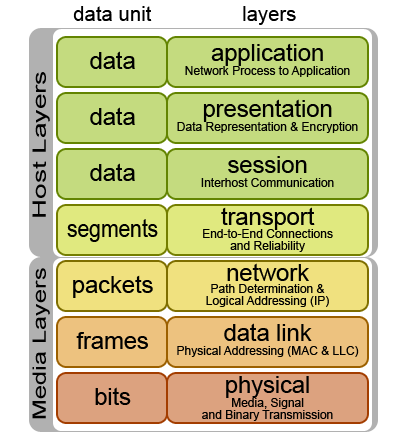
\includegraphics[scale=0.7]{images/OSI-model.png}\\[1cm]
\end{center}


\subsection{Interfaces and Protocols}

\begin{description}
	\item[Interfaces] Interfaces connect different layers on the same computer. Uses Protocol Data Units (PDU).
	\item[Protocols] Protocols are used to communicate between parties data on a specific layer. Uses Service Data Units (SDU) inside Service Access Points (SAP).
\end{description}


\subsection{Encapsulation and Multiplexing}

\begin{description}
	\item[Encapsulation] When data units go down one level in the layer model, headers are added to add information regarding the current layer.
	\item[Multiplexing] Multiple protocols can coexist on the same layer. However, when going down the layer model, these protocols should be treated equally. For example, TCP and UDP are multiplexed down at the IP level, and demultiplexed back when reading the information of IP packets.\footnote{\url{http://www.tcpipguide.com/free/t_TCPIPProcessesMultiplexingandClientServerApplicati-2.htm}}
\end{description}


\subsection{ES Models: Strong vs Weak}

\begin{description}
	\item[Strong ES Model] Hosts suppress packets with a destination address that references another of its interfaces.
	\item[Weak ES Model] Hosts accept packets that match with one of its interfaces addresses, even if it does not receive it on that interface.
\end{description}


\subsection{IP Addressing (IPv4)}

\begin{itemize}
	\item 32-bit addresses
	\item Decimal-dotted notation (a.b.c.d, 0 $=<$ a,b,c,d $=<$ 255).
	\item Special addresses:
	\begin{description}
		\item[0.0.0.0] IP address unknown.
		\item[127.0.0.1] Loopback address.
		\item[Host part all 0] Subnet identifier.
		\item[Host part all 1] Directed broadcast.
		\item[255.255.255.255] Local subnet broadcast.
	\end{description}
	\item Private addresses:
	\begin{description}
		\item[10.0.0.0/8] 
		\item[172.16.0.0/12]
		\item[192.168.0.0/16]
		\item[169.254.0.0/16]
	\end{description}
\end{itemize}


\subsection{Subnetting}

\begin{itemize}
	\item Originally classful subnetting (subnets in A/B/C ranges, with 24, 16 and 8 bits of network addresses respectively; D range for multicast and an unused E range).\footnote{\url{http://en.wikipedia.org/wiki/Classful_network#Introduction_of_address_classes}}
	\item Classless Inter-Domain Routing (CIDR), with network masks to mark the difference between network address and host address. Routing done by selecting most specific match.
	\item Variable Length Subnet Masks (VLSM) to use different subnets that do not have the requirement of having the same size. Add the possibility of subnets inside subnets. This was not possible in RIPv1.
	\item A "link" is defined as the topological area in which a packet with $TTL=1$ can be delivered (aka. not being forwarded).
	\item A "subnet" is the topological area in which the interfaces receive the same network prefix.
\end{itemize}


\subsection{IP Packet Format}

\begin{center}
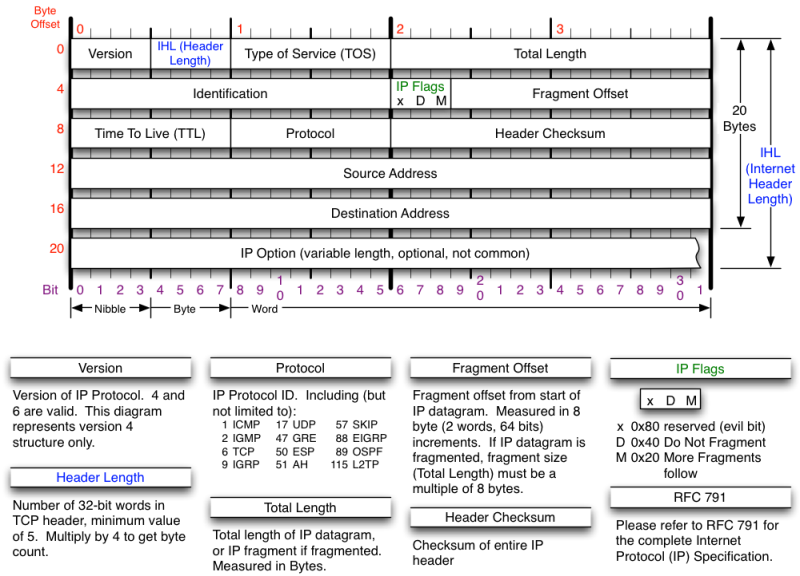
\includegraphics[scale=0.7]{images/IP-Header.png}\\[1cm]
\end{center}

\newpage







\section{CLEAN: Calculating, Legacy, Endianness, Addressing, Networks}

\subsection{Calculating: Counting}

\begin{description}
	\item[Counting] Process that starts with $n=0$ as the initial count. Every counted object is labeled with the actual $n$ value, and n is updated to $n=n+1$. Process ends when all objects have been counted.
\end{description}
	
	
\subsection{Legacy}

\begin{itemize}
	\item Everybody knows what Karst thinks of legacy.
\end{itemize}


\subsection{2-adic vs Binary}

\begin{center}
  \begin{tabular}{ c | c | c | c }
    2-adic & Binary & 2-adic to base-10 & Binary to base-10 \\ \hline
    1 & 0 & 1 & 0 \\ \hline
    2 & 1 & 2 & 1 \\ \hline
    11 & 00 & 3 & 0 \\ \hline
    12 & 01 & 4 & 1 \\ \hline
    21 & 10 & 5 & 2 \\ \hline
    22 & 11 & 6 & 3 \\ \hline
    111 & 000 & 7 & 0 \\ 
    \hline
  \end{tabular}
\end{center}

\begin{itemize}
	\item The whole point is that binary resets at every range increase.
\end{itemize}


\subsection{Big-endian and Little-endian}

\begin{center}
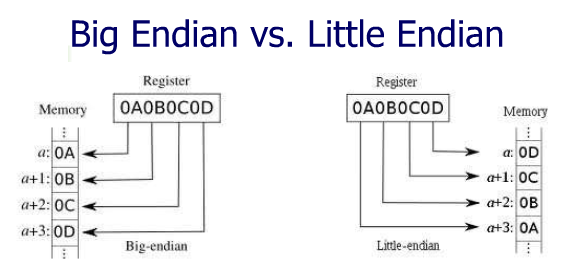
\includegraphics[scale=0.5]{images/BI-LI.png}\\[1cm]
\end{center}


\subsection{Addressing}

\begin{itemize}
	\item \url{http://www.exploringbinary.com/binary-converter/}
\end{itemize}


\newpage







\section{IPv6}


\subsection{Rationale}

\begin{itemize}
	\item $4x$ address space size increase $=$ $2^{96}$ address number increase.
	\item Headers have a fixed size of 40 bytes. Supports extended headers for additional functionality.
	\item NATs no longer needed due the vast amount of addresses.
\end{itemize}


\subsection{Addressing}

\begin{itemize}
	\item 128-bit addresses.
	\item 8 blocks of 4 nibbles ($8x4x4 = 128$ bits)
	\item Consecutive blocks of all-zeroes can be replaced by $::$ once.
	\item No broadcasts, no subnet masks.
	\item \url{http://www.iana.nl/assignments/ipv6-address-space/ipv6-address-space.xhtml}
\end{itemize}


\printbibliography

\end{document}
